

\documentclass[nohyperref]{article}

% Recommended, but optional, packages for figures and better typesetting:
\usepackage{microtype}
\usepackage{graphicx}
%\usepackage{subfigure}
\usepackage{booktabs} % for professional tables

% hyperref makes hyperlinks in the resulting PDF.
% If your build breaks (sometimes temporarily if a hyperlink spans a page)
% please comment out the following usepackage line and replace
% \usepackage{icml2023} with \usepackage[nohyperref]{icml2023} above.
\usepackage{hyperref}


% Attempt to make hyperref and algorithmic work together better:
\newcommand{\theHalgorithm}{\arabic{algorithm}}

% Use the following line for the initial blind version submitted for review:
%remove accepted for blind review
\usepackage[accepted]{icml2023}

% If accepted, instead use the following line for the camera-ready submission:
% \usepackage[accepted]{icml2023}

% For theorems and such
\usepackage{amsmath}
\usepackage{amssymb}
\usepackage{mathtools}
\usepackage{amsthm}

% if you use cleveref..
\usepackage[capitalize,noabbrev]{cleveref}

% my own packages
\usepackage{longtable}

\usepackage{subcaption}
\usepackage[export]{adjustbox}
%\usepackage{subfigure}
\usepackage{caption}
\usepackage{tikz}
\usetikzlibrary{bayesnet}
\usepackage{multirow}
\usepackage{longtable}
\usepackage{makecell}
\usepackage{tikzscale}

%%%%%%%%%%%%%%%%%%%%%%%%%%%%%%%%
% THEOREMS
%%%%%%%%%%%%%%%%%%%%%%%%%%%%%%%%
\theoremstyle{plain}
\newtheorem{theorem}{Theorem}[section]
\newtheorem{proposition}[theorem]{Proposition}
\newtheorem{lemma}[theorem]{Lemma}
\newtheorem{corollary}[theorem]{Corollary}
\theoremstyle{definition}
\newtheorem{definition}[theorem]{Definition}
\newtheorem{assumption}[theorem]{Assumption}
\theoremstyle{remark}
\newtheorem{remark}[theorem]{Remark}

\usepackage[textsize=tiny]{todonotes}

\newcommand{\cblock}[3]{
 %\hspace{-1.5mm}
 \begin{tikzpicture}
   [
   node/.style={square, minimum size=10mm, thick, line width=0pt, anchor=center, align=center},
   ]
   \node[fill={rgb,255:red,#1;green,#2;blue,#3}] () [] {};
 \end{tikzpicture}%
}

\newcommand{\cstar}[3]{
  \begin{tikzpicture}[scale=0.5]
    \node[star,star points=5,star point ratio=2.5,          minimum size=10mm,thick,          fill={rgb,255:red,#1;green,#2;blue,#3}] () [] {};
  \end{tikzpicture}%
}




% Todonotes is useful during development; simply uncomment the next line
%    and comment out the line below the next line to turn off comments
%\usepackage[disable,textsize=tiny]{todonotes}
\usepackage[textsize=tiny]{todonotes}


% The \icmltitle you define below is probably too long as a header.
% Therefore, a short form for the running title is supplied here:
\icmltitlerunning{Training Language Models with Language Feedback at Scale}

\begin{document}
%\setlength{\abovedisplayskip}{-5pt}
%\setlength{\belowdisplayskip}{5pt}
%\setlength{\abovedisplayshortskip}{-10pt}
%\setlength{\belowdisplayshortskip}{pt}
\twocolumn[
\icmltitle{Training Language Models with Language Feedback at Scale}

% It is OKAY to include author information, even for blind
% submissions: the style file will automatically remove it for you
% unless you've provided the [accepted] option to the icml2023
% package.

% List of affiliations: The first argument should be a (short)
% identifier you will use later to specify author affiliations
% Academic affiliations should list Department, University, City, Region, Country
% Industry affiliations should list Company, City, Region, Country

% You can specify symbols, otherwise they are numbered in order.
% Ideally, you should not use this facility. Affiliations will be numbered
% in order of appearance and this is the preferred way.
\icmlsetsymbol{equal}{*}

\begin{icmlauthorlist}
\icmlauthor{Jérémy Scheurer}{nyu,far}
\icmlauthor{Jon Ander Campos}{nyu,ba}
\icmlauthor{Tomasz Korbak}{nyu,far,su}
\icmlauthor{Jun Shern Chan}{nyu,far}
\icmlauthor{Angelica Chen}{nyu}
\icmlauthor{Kyunghyun Cho}{nyu,gen,cif}
\icmlauthor{Ethan Perez}{nyu,far,ant}
\end{icmlauthorlist}

\icmlaffiliation{nyu}{New York University}
\icmlaffiliation{far}{FAR AI}
\icmlaffiliation{ba}{HiTZ Center, University of the Basque Country UPV/EHU}
\icmlaffiliation{su}{University of Sussex}
\icmlaffiliation{gen}{Genentech}
\icmlaffiliation{cif}{CIFAR LMB}
\icmlaffiliation{ant}{Anthropic}


\icmlcorrespondingauthor{Jérémy Scheurer}{jeremy.scheurer@nyu.edu}
\icmlcorrespondingauthor{Ethan Perez}{ethan@anthropic.com}

% You may provide any keywords that you
% find helpful for describing your paper; these are used to populate
% the "keywords" metadata in the PDF but will not be shown in the document
\icmlkeywords{Language Models, Bayesian Inference, Reinforcement Learning from Human Feedback}

\vskip 0.3in
]

% this must go after the closing bracket ] following \twocolumn[ ...

% This command actually creates the footnote in the first column
% listing the affiliations and the copyright notice.
% The command takes one argument, which is text to display at the start of the footnote.
% The \icmlEqualContribution command is standard text for equal contribution.
% Remove it (just {}) if you do not need this facility.

%\printAffiliationsAndNotice{}  % leave blank if no need to mention equal contribution
%\printAffiliationsAndNotice{\icmlEqualContribution} % otherwise use the standard text.

\printAffiliationsAndNotice{}

\begin{abstract}
Pretrained language models often generate outputs that are not in line with human preferences, such as harmful text or factually incorrect summaries. Recent work approaches the above issues by learning from a simple form of human feedback: comparisons between pairs of model-generated outputs. However, comparison feedback only conveys limited information about human preferences. In this paper, we introduce Imitation learning from Language Feedback (ILF), a new approach that utilizes more informative language feedback. ILF consists of three steps that are applied iteratively: first, conditioning the language model on the input, an initial LM output, and feedback to generate refinements. Second, selecting the refinement incorporating the most feedback. Third, finetuning the language model to maximize the likelihood of the chosen refinement given the input. We show theoretically that ILF can be viewed as Bayesian Inference, similar to Reinforcement Learning from human feedback. We evaluate ILF's effectiveness on a carefully-controlled toy task and a realistic summarization task.
Our experiments demonstrate that large language models accurately incorporate feedback and that finetuning with ILF scales well with the dataset size, even outperforming finetuning on human summaries. Learning from both language and comparison feedback outperforms learning from each alone, achieving human-level summarization performance. 
\end{abstract}
%Pretrained language models often do not perform tasks in ways that are in line with our preferences, e.g., they generate harmful text or factually incorrect summaries. Recent work approaches the above issue by learning from a simple form of human evaluation: comparisons between pairs of model-generated task outputs. However, comparison feedback can only convey limited information about human preferences. Here, we propose \textbf{i}mitation learning from \textbf{l}anguage \textbf{f}eedback (ILF), a new approach that utilises more informative language feedback.
%ILF consists of three steps that we iteratively apply: first, we condition the language model on the initial output and feedback to generate many refinements.
%Second, we choose the refinement incorporating most of the feedback.
%Third, we finetune a language model to maximize the likelihood of the chosen refinement given the input.
%We formally demonstrate that ILF can be viewed as Bayesian Inference, and we evaluate its effectiveness on synthetic data and a new preference learning dataset called SLF-5K. Our experiments show that large language models are able to accurately incorporate feedback to generate refinements and that finetuning with ILF scales well with the size of the dataset, even outperforming finetuning on human summaries. Additionally, we find that while learning from binary comparisons is more sample efficient than learning from language feedback, combining ILF with a reward model trained on binary comparisons produces the best results and achieves roughly human-level summarization ability.

%Alternative abstarct
%Language models have the potential to significantly improve our ability to perform a wide range of tasks, but they often do not align with our preferences. For example, they may generate harmful text or factually incorrect summaries. In this paper, we propose Imitation Learning from Language Feedback (ILF) as a solution to this problem. ILF allows language models to learn from more informative language feedback, rather than just simple comparisons between pairs of outputs. By iteratively applying three steps - generating refinements using the initial output and feedback, choosing the refinement that best incorporates the feedback, and finetuning the language model on the chosen refinement - we can effectively teach language models to align with our preferences. We demonstrate the effectiveness of ILF on synthetic data and a new preference learning dataset called SLF-5K, and show that it scales well with the size of the dataset. In fact, ILF outperforms finetuning on human summaries in some cases. Additionally, we find that combining ILF with a reward model trained on binary comparisons produces the best results, achieving roughly human-level summarization ability. Our work represents a major step forward in the ability of language models to learn from human preferences.

\section{Introduction}
\label{sec:introduction}
% \begin{itemize}
%     % Diffusion of FL
%     \item {\st{Diffusion of FL}}
%     % Security threats to FL
%     \item {\st{Security threats to FL with particular focus on model poisoning}}
%     % Limitations of existing countermeasures
%     \item {\st{Current countermeasures (e.g., KRUM) and their limitations}}
%     % Proposed method and its advantages
%     \item {\st{Intuitive description of the proposed method and its difference (i.e., advantages) w.r.t. state of the art}}
%     % Main contributions
%     \item {\st{Summary of the main contributions of this work}}
%     % Paper's structure and organization
%     \item {\st{Paper's structure and organization}}
% \end{itemize}

% Diffusion of FL
Recently, {\em federated learning} (FL) has emerged as the leading paradigm for training distributed, large-scale, and privacy-preserving machine learning (ML) systems~\cite{mcmahan2017googleai,mcmahan2017aistats}. 
The core idea of FL is to allow multiple edge clients to collaboratively train a shared, global model without disclosing their local private training data.
%Specifically, an FL system consists of a central server and many edge clients; 
A typical FL round involves the following steps: {\em(i)} the server randomly picks some clients and sends them the current, global model; {\em(ii)} each selected client locally trains its model with its own private data; then, it sends the resulting local model to the server;\footnote{Whenever we refer to global/local model, we mean global/local model {\em parameters}.} {\em(iii)} the server updates the global model by computing an \emph{aggregation function}, usually the average (FedAvg), on the local models received from clients.
% \begin{enumerate}
%     \item[{\em(i)}] the server sends the current, global model to the clients and appoints some of them for training;
%     \item[{\em(ii)}] each selected client locally trains its copy of the global model with its own private data; then, it sends the resulting local model back to the server;\footnote{Whenever we refer to global/local model, we mean global/local model {\em parameters}.}
%     \item[{\em(iii)}] the server updates the global model by computing an \emph{aggregation function} on the local models received from clients (by default, the average, also referred to as FedAvg~\cite{mcmahan2017aistats}).
% \end{enumerate}
This process goes on until the global model converges. %(e.g., after a certain number of rounds or other similar stopping criteria).
%\\
% The advantages of FL over the traditional, centralized learning paradigm are undoubtedly clear in terms of flexibility/scalability (clients can join/disconnect from the FL network dynamically), network communications (only model weights\footnote{We will use \textit{parameters} and \textit{weights} interchangeably.} are exchanged between clients and server), and privacy (each client's private training data is kept local at the client's end and not uploaded to the server).
\\
% Security threats to FL
%However, the growing adoption of FL also raises security concerns~\cite{costa2022covert}, particularly about its confidentiality, integrity, and availability.
Although its advantages over standard ML, FL also raises security concerns~\cite{costa2022covert}. %, particularly about its confidentiality, integrity, and availability~\cite{costa2022covert}.
% OLD, LONG VERSION
% Indeed, some work deals with privacy leakage that may expose the local data of some clients~\cite{melis2019sp}. 
% A large body of work, instead, investigates attacks that usually aim to detriment the predictive accuracy of the learned global model. For instance, \emph{data poisoning} attacks achieve this goal by letting an adversary pollute the training set of some corrupt FL clients with maliciously crafted examples~\cite{jagielski2018sp}.
% Similarly, in \emph{model poisoning} the attacker attempts to tweak the global model weights~\cite{bhagoji2019pmlr} by directly perturbing the local model's weights of some infected FL clients before these are sent to the central server for aggregation, usually via so-called Byzantine attacks. 
% It turns out that Byzantine model poisoning attacks severely impact standard FedAvg; therefore, more robust aggregation functions must be designed to make FL systems secure.
Here, we focus on \emph{untargeted model poisoning} attacks~\cite{bhagoji2019pmlr}, where an adversary attempts to tweak the global model weights %\footnote{We will use the terms \textit{parameters} and \textit{weights} interchangeably.} 
by directly perturbing the local model's parameters of some infected clients before these are sent to the central server for aggregation.
In doing so, the adversary aims to jeopardize the global model \textit{indiscriminately} at inference time.
Such model poisoning attacks severely impact standard FedAvg; therefore, more robust aggregation functions must be designed to secure FL systems.
\\
% In this paper, we focus on designing a novel robust aggregation scheme at the server's end to contrast the effect of Byzantine model poisoning attacks.
%
% Current countermeasures and their limitations
%Several countermeasures have been proposed in the literature to combat model poisoning attacks on FL systems.
% Some methods use simple statistics more robust than plain average to smooth the impact of malicious updates (e.g., Trimmed Mean and FedMedian~\cite{yin2018icml}). 
% Other defenses implement outlier detection techniques to discard malicious updates from the aggregation performed at the server's end. Those are either based on heuristics (e.g., Krum/Multi-Krum~\cite{blanchard2017nips} and Bulyan~\cite{mhamdi2018pmlr}) or data-driven approaches (e.g., K-means clustering~\cite{shen2016acm} or DnC via spectral analysis~\cite{shejwalkar2021ndss}). 
% Finally, some strategies rely on a centralized ``source of trust'' to spot potential malicious updates (e.g., FLTrust~\cite{cao2020fltrust}).
% Several countermeasures have been proposed in the literature to combat model poisoning attacks on FL systems, i.e., to discard possible malicious local updates from the aggregation performed at the server's end. 
% These techniques range from simple statistics more robust than plain average (e.g., Trimmed Mean and FedMedian~\cite{yin2018icml}) to outlier detection heuristics (e.g., Krum/Multi-Krum~\cite{blanchard2017nips} and Bulyan~\cite{mhamdi2018pmlr}) or data-driven approaches (e.g., spectral analysis via K-means clustering~\cite{shen2016acm} or spectral analysis), or methods based on ``source of trust'' (e.g., FLTrust~\cite{cao2020fltrust}).
% OLD, LONG VERSION
%Several countermeasures have been proposed in the literature to combat Byzantine model poisoning attacks on FL systems.
% Descriptive statistics
% For example, Trimmed Mean and FedMedian aggregate local model updates using more robust statistics than standard average~\cite{yin2018icml}.
%
% % Heuristics for outlier detection
% Many existing Byzantine-resilient strategies implement some outlier detection heuristics to discard the model updates sent by potentially malicious clients from the input of the aggregation function.
% One of the most popular heuristics is Krum~\cite{blanchard2017nips}.
% This strategy tries to mitigate the impact of Byzantine attacks by selecting as a global model the local model with the smallest sum of Euclidean distances to {\em all} the other local models.
% Although powerful, Krum requires the server to know (or, at least, estimate) the number of malicious FL clients upfront, which is generally impossible in a realistic attack scenario. %
% Moreover, Krum may become ineffective for complex, high-dimensional model parameter spaces due to the curse of dimensionality.
% Bulyan~\cite{mhamdi2018pmlr} tries to overcome this issue by combining Krum with a variant of Trimmed Mean.
% % Data-driven outlier detection
% Other strategies use data-driven outlier detection techniques -- e.g., via K-means clustering~\cite{shen2016acm} -- to spot potential malicious local model updates. 
% %For instance, Shen et al. propose to cluster local model updates with K-means and thus identify outliers.
%
% % Other techniques
% As far as the server is concerned, any local model received can be from a potential malicious client. 
% FLTrust~\cite{cao2020fltrust} assumes the server acts as a client, i.e., trains a local model on an additional {\em trustworthy} dataset at the server's end and compares it against all the local models from other clients. 
% This way, the server can rely on some ``source of trust'' when discarding potentially malicious clients.
%\\
% Limitations of existing Byzantine-resilient strategies
Unfortunately, existing defense mechanisms either rely on simple heuristics (e.g., Trimmed Mean and FedMedian by~\cite{yin2018icml}) or need strong and unrealistic assumptions to work effectively (e.g., foreknowledge or estimation of the number of malicious clients in the FL system, as for Krum/Multi-Krum~\cite{blanchard2017nips} and Bulyan~\cite{mhamdi2018pmlr}, which, however, cannot exceed a fixed threshold).
Furthermore, outlier detection methods using K-means clustering~\cite{shen2016acm} or spectral analysis like DnC~\cite{shejwalkar2021ndss} do not directly consider the temporal evolution of local model updates received.
Finally, strategies like FLTrust~\cite{cao2020fltrust} require the server to collect its own dataset and act as a proper client, thereby altering the standard FL protocol.
\\
% OLD, LONG VERSION
% Overall, existing Byzantine-resilient strategies are either simple heuristics (e.g., FedMedian) or, if they are more complex, they rely on strong and unrealistic assumptions to work effectively (e.g., knowing the number of malicious clients in the FL system in advance, as for Krum and alike).
% Furthermore, data-driven outlier detection methods do not consider the temporary evolution of local model updates received (e.g., K-means clustering). 
% Finally, strategies like FLTrust requires the server to collect its own dataset and act as a proper client, thereby altering the standard FL protocol.
%
% Description of the proposed method
This work introduces a novel pre-aggregation \textit{filter} robust to untargeted model poisoning attacks. Notably, this filter $(i)$ operates without requiring prior knowledge or constraints on the number of malicious clients and $(ii)$ inherently integrates temporal dependencies. 
The FL server can employ this filter as a preprocessing step before applying \textit{any} aggregation function, be it standard like FedAvg or robust like Krum or Bulyan.
Specifically, we formulate the problem of identifying corrupted updates as a multidimensional (i.e., matrix-valued) time series anomaly detection task. 
The key idea is that legitimate local updates, resulting from well-calibrated iterative procedures like stochastic gradient descent (SGD) with an appropriate learning rate, show \textit{higher predictability} compared to malicious updates. This hypothesis stems from the fact that the sequence of gradients (thus, model parameters) observed during legitimate training exhibit regular patterns, as validated in Section~\ref{subsec:intuition}. %until convergence. 
%This regularity may be more pronounced for smooth convex loss functions, but it can still be captured within an appropriate time window, even for more complex and convoluted loss surfaces. 
%We provide evidence of this claim in Appendix~B, where we show that the average mutual information (i.e., ``predictability''), calculated over pairs of legitimate model updates sent at different FL rounds, is significantly higher than the corresponding computation for a malicious client.
\\
Inspired by the matrix autoregressive (MAR) framework for multidimensional time series forecasting~\cite{chen2021je}, we propose the FLANDERS ({\em \textbf{F}ederated \textbf{L}earning meets \textbf{AN}omaly \textbf{DE}tection for a \textbf{R}obust and \textbf{S}ecure}) filter.
The main advantages of FLANDERS over existing strategies like FLDetector~\cite{zhao2020multivariate} are its resilience to large-scale attacks, where $50\%$ or more FL participants are hostile, and the capability of working under realistic non-iid scenarios.
We attribute such a capability to two key factors: $(i)$ FLANDERS works without knowing a priori the ratio of corrupted clients, and $(ii)$ it embodies temporal dependencies between intra- and inter-client updates, quickly recognizing local model drifts caused by evil players. Below, we summarize our main contributions:

\begin{itemize}
\item[{\em(i)}]
We provide empirical evidence that the sequence of models sent by legitimate clients is more predictable than those of malicious participants performing untargeted model poisoning attacks.
\\
\item[{\em(ii)}] 
We introduce FLANDERS, the first pre-aggregation filter for FL robust to untargeted model poisoning based on multidimensional time series anomaly detection.
\\
\item[{\em(iii)}] 
We integrate FLANDERS into Flower,\footnote{\scriptsize{\url{https://flower.dev/}}} a popular FL simulation framework for reproducibility.
\\
\item[{\em(iv)}] 
We show that FLANDERS improves the robustness of the existing aggregation methods under multiple settings: different datasets, client's data distribution (non-iid), models, and attack scenarios.
\\
\item[{\em(v)}] 
We publicly release all the implementation code of FLANDERS along with our experiments.\footnote{\scriptsize{\url{https://anonymous.4open.science/r/flanders_exp-7EEB}}}
\end{itemize}

% Paper's structure and organization
The remainder of the paper is structured as follows. %some related work and the current state-of-the-art solutions to security issues that FL entails. 
Section~\ref{sec:background} covers background and preliminaries. 
In Section~\ref{sec:related}, we discuss related work.
Section~\ref{sec:problem} and Section~\ref{sec:method} describe the problem formulation and the method proposed. % to tackle it. 
Section~\ref{sec:experiments} gathers experimental results. %, and Section~\ref{sec:limitations} discusses some limitations of this work.
Finally, we conclude in Section~\ref{sec:conclusion}.
 %discusses the limitations of this work and draws future research directions.
%reports conclusions and draws perspectives for future research directions.

%%%%%%% OLD %%%%%%%
%to overcome the resilience of Byzantine failures in distributed Stochastic Gradient Descent computations. 
% The strength of Krum is its time complexity, which is linear in the gradient dimension. 
% However, the robustness of the approach is guaranteed for gradient-based learning applications only when the majority of the clients are not compromised. 
% Besides, the aggregation mechanism of Krum, as well as that of similar methods, is robust from a coarse-grained perspective and does not provide solutions to errors and perturbations that may occur at inference time.
%A related approach to~\cite{blanchard2017nips} is the work of Su et al.~\cite{su2016dc}. Here, the authors propose an iterated approximate agreement to tackle a multi-layer scenario attacked by Byzantine agents. 
%However, the method works efficiently on the sole discrete context and it is inapplicable to continuous state environments.
%\gabri{Maybe, we should just talk about the main limitations of existing countermeasures without digging into their details (or, we can just mention Krum as this is the most popular one). I will move the description of all these methods to the Related Work section.}
\section{PoseRAC Model}
\label{sec4}

\begin{figure*}[t]
\centering
\includegraphics[width=1.0\textwidth]{figure5.pdf}
\caption{Overview of our proposed PoseRAC. For a input video, the repetitive count can be obtained through Pose Estimation, Transformer Encoder, Pose Mapping and Action-trigger, where only the Encoder and the Pose Mapping need to be trained. We use Triplet Margin Loss to train the Encoder while Binary Cross Entropy Loss to train both the Encoder and the Pose Mapping. In addition to achieving the state-of-the-art performance so far, the biggest highlight of our PoseRAC is that it is lightweight enough to be easily trained on a CPU.}
\label{fig5}
\end{figure*}

Given a video $V={\{x_i\}}^{T}_{1}\in \mathbb{R}^{C\times H\times W\times T}$ with $T$ RGB frames, repetitive action counting model aims to predict a certain value $Y$, which is the number of repetitive actions. In this section, we will introduce our PoseRAC in detail.

\subsection{Model Overview}

As shown in Figure \ref{fig5}, PoseRAC consists of four parts. 

\begin{itemize}

\item The first is a state-of-the-art and lightweight Pose Estimation Network~($\S\ref{first}$), which is used to estimate the poses represented by lots of human pose key points from each frame of the original video sequence. 

\item The second is a simple Transformer Encoder~($\S\ref{second}$) to embed the key points of poses into high-level feature space, where the same class have similar distances, while the distances of different classes are far apart.

\item The third is a Pose Mapping Module~($\S\ref{third}$), where the unique mapping relationship between the salient poses and the action classes can be learned. Each pose can be mapped to the action class with the highest probability after the previous encoding.

\item The fourth part is a lightweight Action-trigger Module~($\S\ref{fourth}$). When we get the salient action classification results of all frames of the entire video sequence, we can use this module to calculate the repetition count in a short time.

\end{itemize}

\subsection{Pose Estimation Network}
\label{first}
Our model first converts the video sequence into a sequence of human pose key points, which can be defined as: 
\begin{equation}
\begin{split}
&V={\{x_i\}}^{T}_{1}\in \mathbb{R}^{C\times H\times W\times T}\\
&V\xrightarrow{\mathrm{Pose Estimation}} P={\{p_i\}}^{T}_{1}\in \mathbb{R}^{D\times K\times T}
\end{split}
\label{eq1}
\end{equation}
where each $x_i$ represents a single RGB frame, and each $p_i$ represents the key points of each frame. To express the key points of each frame, we use $D\times K$ sequence, which includes two parts, one ($K$) is the number of key points to fully represent the current pose, the other ($D$) is the dimension of each key point, generally three, which are the two coordinates of the planes and the depth estimation.

Here we use state-of-the-art pose estimation models such as Vitpose\cite{xu2022vitpose} and BlazePose\cite{bazarevsky2020blazepose}. The pose estimation algorithms themselves are not designed by us, but we introduce pose information into the action counting task, which is a novel design not explored by previous work.

Moreover, our pose-level poses estimation processes the primitive information of video, which is similar to the feature extraction network in all video-level algorithms such as I3D\cite{carreira2017quo}, VideoSwinTransformer\cite{liu2022video}, and TSN\cite{wang2016temporal}. But the difference is that the result of video-level incorporates all information, while pose-level only produces core information, which greatly improves the performance. Additionally, using pose information can contribute to the lightweight of model. For instance, for a 1024-frame video, video-level feature extraction with an output dimension of 512 would produce a data volume of $1024\times 512=524288$, while using pose information with 33 key points produces a data volume of only $1024\times 33 \times 3=101376$.

\subsection{Encoding Poses with Transformer}
\label{second}
Here we specify our data representation for the Transformer Encoder, which requires input batch size, sequence length, and embedding dimensions. In our pose-level approach, each frame is a batch, the number of key points in each frame is the sequence length, and the feature dimension of each key point is the embedding dimension.

First we get the pose of each frame ${p_i}\in \mathbb{R}^{D\times K}$ through the Pose Estimation Network, where $i\in {1, 2, \dots, T}$ is the frame index, $K$ is the number of key points, and $D$ is the dimension of each key point. We further define $p_i = {\{k_j\}}^{K}_{1}$ to represent each key point, where $k_j\in \mathbb{R}^D$, and we embed it to obtain richer information. Our embedding projection $\mathrm{\bf{E}}$ is a simple MLP network with ReLU as the activation function. These calculations can be defined as:
\begin{equation}
\begin{split}
\mathrm{\bf{Z}}^0 = [\mathrm{\bf{E}}(k_1), \mathrm{\bf{E}}(k_2), \dots, \mathrm{\bf{E}}(k_K)]^T
\end{split}
\end{equation}
where $\mathrm{\bf{E}}(k_j)\in \mathbb{R}^{D^{\prime}}$ is the embedding feature. Then the next Transformer takes $\mathrm{\bf{Z}}^0$ as input and encodes it with self-attention. Given $\mathrm{\bf{Z}}^0\in \mathbb{R}^{K\times D^{\prime}}$ with $K$ key point features, each of which is $D^{\prime}$-dimensional, $\mathrm{\bf{Z}}^0$ is projected using $\mathrm{\bf{W}}_Q\in \mathbb{R}^{D^{\prime}\times D_q}$, $\mathrm{\bf{W}}_K\in \mathbb{R}^{D^{\prime}\times D_k}$, $\mathrm{\bf{W}}_V\in \mathbb{R}^{D^{\prime}\times D_v}$, where $D_k=D_q$, to extract feature representations query($\mathrm{\bf{Q}}$), key($\mathrm{\bf{K}}$) and value($\mathrm{\bf{V}}$), which can be defined as:
\begin{equation}
\begin{split}
&\mathrm{\bf{Q}}=\mathrm{\bf{Z}}^0\times \mathrm{\bf{W}}_Q\\
&\mathrm{\bf{K}}=\mathrm{\bf{Z}}^0\times \mathrm{\bf{W}}_K\\
&\mathrm{\bf{V}}=\mathrm{\bf{Z}}^0\times \mathrm{\bf{W}}_V
\end{split}
\end{equation}
and the output of self-attention can be computed as:
\begin{equation}
\begin{split}
\mathrm{\bf{Attn}}=\mathrm{Softmax}(\frac{\mathrm{\bf{Q}}\mathrm{\bf{K}}^T}{\sqrt{D_q}})\mathrm{\bf{V}}
\end{split}
\end{equation}
where $\mathrm{\bf{Attn}}\in \mathbb{R}^{K\times D^{\prime}}$. Also, we use common multi-head self-attention (MHSA) to make several self-attention operations calculate in parallel.

Now we introduce the overall architecture of Transformer Encoder, which has $L$ layers with each layer consisting of MHSA and MLP blocks. Also, LayerNorm and Residual Connection are applied before and after every MHSA or MLP block, respectively. Because the number of key points of each frame is  a bit less, so our encoder does not include the downsampling module that other models may have. The overall process can be defined as:
\begin{equation}
\begin{split}
&\mathrm{\bf{\hat{Z}}}^l = \mathrm{MHSA}(\mathrm{LN}(\mathrm{\bf{Z}}^{l-1})) + \mathrm{\bf{Z}}^{l-1}\\
&\mathrm{\bf{Z}}^l = \mathrm{MLP}(\mathrm{LN}(\mathrm{\bf{\hat{Z}}}^l)) + \mathrm{\bf{\hat{Z}}}^l
\end{split}
\end{equation}
where $\mathrm{\bf{Z}}^{l-1}$, $\mathrm{\bf{\hat{Z}}}^l$, $\mathrm{\bf{Z}}^l\in \mathbb{R}^{K\times D^{\prime}}$.


\subsection{Pose Mapping}
\label{third}
Taking the Encoder output $\mathrm{\bf{Z}}^L\in \mathbb{R}^{K\times D^{\prime}}$ as input, Pose Mapping module outputs probability scores $\mathrm{\bf{S}}\in \mathbb{R}^{C}$ of the current frame over all action classes. We perform binary classification after Sigmoid activation for each class, with the two salient poses of each class represented by the same bit data. To realize such a module, we use a very lightweight MLP network, which avoids the complexity. First, the two dimensions $K$ and $D^{\prime}$ of $\mathrm{\bf{Z}}^L$ are flattened into $\mathbb{R}^{KD^{\prime}}$, and then it passes through an MLP module, where the output channels is set to $C$, which can be defined as:
\begin{equation}
\begin{split}
\mathrm{\bf{S}} = \sigma(\mathrm{MLP}(\mathrm{Flatten}(\mathrm{\bf{Z}}^L)))
\end{split}
\end{equation}
where $\sigma$ represents the Sigmoid activation function.

With such Pose Mapping, we can obtain the scores of single frame. It should be noted that we extract the poses of all frames, and use the convenience of matrix operations to obtain scores in parallel, which is actually consistent with the idea of mini batch. So at last, we combine the scores of all frames to get the video score matrix $\mathrm{\bf{\hat{S}}}\in \mathbb{R}^{C\times T}$, where $T$ represents the number of frames in the current video. 


\subsection{Action-trigger Module}
\label{fourth}
We use the lightweight Action-trigger Module to obtain the final output $Y$, the repetitive action count, which has a time complexity of $\mathcal{O}(n)$. First, we get the scores $S_c\in \mathbb{R}^T$ of a given action class from $\mathrm{\bf{\hat{S}}}$. Then, we scan all frames and use the action-trigger mechanism to count when the two salient poses of the action class occur sequentially. We set upper and lower bounds to distinguish the scores of the two salient poses, which cluster non-salient poses in the middle and easily classify the salient poses to the two ends.

\subsection{Losses and Metric Learning}

The modules need to be trained are Embedding, Transformer Encoder and Pose Mapping, and because we perform binary classification for each class, so we use the Binary Cross Entropy Loss, which can be defined as follows:
\begin{gather}
\mathcal{L}_{bce} = -\frac{1}{N}\sum\limits_{i=1}^{N}(\frac{1}{C}\sum\limits_{j=1}^{C}loss(i,j))  \\
 loss(i,j)=y_{ij}\log p_{ij} + (1-y_{ij})\log(1-p_{ij})
\end{gather}
where $N$ represents the batch size (in our method, each frame is a batch), $C$ represents the number of classes, $y$ and $p$ are the labels and our predictions, respectively.

Moreover, we use Metric Learning to improve our Encoder and introduce the Pose Triplet Loss. Given a pose, Encoder produces higher-level features $\mathrm{\bf{Z}}^L$, which should be more representative. As shown in Figure \ref{fig5}, we achieve this with Triplet Margin Loss function, which selects anchors, same class positive samples, and different classes negative samples in a batch. It can be expressed as:
\begin{equation}
\begin{split}
\mathcal{L}_{tri} = \mathrm{max}(\mathrm{CS}(a,p)-\mathrm{CS}(a,n)+\mathrm{margin},0)
\end{split}
\end{equation}
where $a$, $p$, $d$ are anchors, positive and negative samples, and $\mathrm{CS}$ represents the Cosine Similarity to measure the distance between features. We pay more attention to hard samples, where the distances between anchors and negative samples are even smaller than those of positive samples. After Metric Learning, the poses of each action can be distinguishable, which cluster in the high-level space.

At last, our overall training combines these two losses:
\begin{equation}
\begin{split}
\mathcal{L} = \mathcal{L}_{bce} + \alpha\mathcal{L}_{tri}
\end{split}
\end{equation}
where $\alpha$ is the weight factor to control the two losses in the same numeric scale.
\subsection{Implementation Details}

\noindent{\bf Training.} We use the \emph{RepCount-pose} and \emph{UCFRep-pose} dataset we created to train our model. Only the frames with salient poses are inputted into the network instead of the entire video to speed up the fitting.

\noindent{\bf Inference.} During inference, the entire video sequence is inputted into the model. The poses of all frames pass through the Encoder and Pose Mapping, and then enter the Action-trigger Module to output the repetitive count.
%\section{Method - Bayesian Inference}
We now formulate the problem setting and describe our approach. We aim to generate improved outputs $x_1$ (e.g., high-quality summaries), according to human preferences, given language feedback $f$ on an initial model-generated output $x_0$, and a context $c$ (e.g., a source document). We tackle this problem by updating an LM $\pi_{\theta}$ based on evidence provided by language feedback.

%In this section we define our problem formally and introduce our algorithm in its most general form. Given a context $c$ we seek to generate an output $x_1$ that is helpful and harmless according to human preference judgments. We assume access to language feedback $f$ on an initial model-generated output $x_0$ given the context $c$. In the following section, we frame this problem as Bayesian inference, i.e. updating an LM $\pi_{\theta}$ based on evidence provided by language feedback. Then we introduce ILF, our algorithm for learning from language feedback. 

\paragraph{Language Feedback as Variational Inference}
Our goal is to produce a high-quality output $x_1$ for a context $c \sim p(c)$ (e.g., a summary of a document). We use an LM $\pi_{\theta}$ to generate an output $x_1$, by conditioning on the context $c$, i.e., $x_1 \sim p_{\theta}(x_1|c)$. We then introduce the predicate $\mathcal{I}$, a random variable such that $\mathcal{I}=1$ if the output is high quality according to human preferences.
We denote this data-generating process, shown in Fig.~\ref{fig:data_generating_process}, as:
\begin{align}
    p_\theta(c, x_1, \mathcal{I}) = p(c) \pi_\theta(x_1|c) p(\mathcal{I}|c,x_1).
\end{align}
%The goal of maximizing summary helpfulness across contexts $c$ can then be framed as maximising the expected probability of helpfulness:
%\begin{align}
%p_\theta(\mathcal{I}=1) &= \mathbb{E}_{c \sim p(c)} p(\mathcal{I}=1|c) \\
%&= \mathbb{E}_{c \sim p(c)} \mathbb{E}_{x_1\sim \pi_\theta(x_1|c)} p(\mathcal{I}=1|c,x_1)
%\end{align}
%If we treat $p(\mathcal{I}=1|c, x_1)$ as a reward, this objective is equivalent to the RL objective of the expected reward. 
%However, instead of using RL, 
We frame our goal as maximizing the marginal log probability of quality across contexts: $\mathbb{E}_{c \sim p(c)} \log p(\mathcal{I}=1|c).$ %
% of generating high-quality summaries as 
% expected log probability of summary quality, i.e., $\mathbb{E}_{c \sim p(c)}  \mathbb{E}_{x_1\sim \pi_\theta(x_1|c)} \log p(\mathcal{I}=1|c,x_1)$.  
For a particular context $c$, we approximate $\log p(\mathcal{I}=1|c)$ by introducing an importance sampling proposal distribution $q(x_1|c)$ and using the Evidence Lower Bound (ELBo):
%We will use the fact that $p(\mathcal{I}=1|c)$ has the following lower bound: 
\begin{align}
\log p(\mathcal{I}=1|c) &= \log \sum_{x_1} p_\theta(x_1, \mathcal{I}=1|c) \label{eq:two} \\
% &= \log \sum_{x_1} q(x_1|c) \frac{p_\theta(x_1, \mathcal{I}=1|c)}{q(x_1|c)} \label{eq:three}\\
&\geq \sum_{x_1} q(x_1|c) \log \frac{p_\theta(x_1, \mathcal{I}=1|c)}{q(x_1|c)} \label{eq:four}
% &= \sum_{x_1} q(x_1|c)  \Big[ \log p_\theta(x_1, \mathcal{I}=1|c) - \log q(x_1|c) \Big] \label{eq:five} \\
%&:= F(\theta, q) \label{eq:six}
\end{align}
%In Eq.~\ref{eq:two}, we use the sum rule, in Eq.~\ref{eq:three}, we introduce an importance sampling proposal distribution $q(x_1|c)$, in Eq.~\ref{eq:four} we use the Jensen inequality and in Eq.~\ref{eq:six} we define $F$, the lower bound to maximize. 

We maximize the lower bound in Eq. \ref{eq:two}, henceforth called $F(\theta, q)$, using an Expectation-Maximization (EM) procedure: alternating between maximizing $F$ w.r.t. the proposal distribution $q$ (E-step) and w.r.t. $\pi_{\theta}$ (M-step)  We call this algorithm Imitation learning from Language Feedback.

 %
% There exists a closed form for such an optimal $q$ (see Appendix~\ref{appendix:optimal_q} for the full derivation):
% \begin{align*}
% \operatorname*{argmax}_q F(\theta, q)
% &= p_\theta(x_1|\mathcal{I}=1,c) \vcentcolon= q^*(x_1|c).
% \end{align*}
% \begin{figure}[t]
%     \centering
%     \begin{subfigure}
%         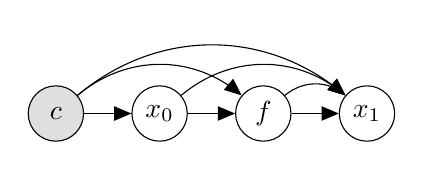
\begin{tikzpicture}
  % Define nodes
  \node[obs]           (c) {$c$};
  \node[latent, right=0.6cm of c]       (x_0) {$x_0$};
  \node[latent, right=0.6cm of x_0]     (f) {$f$};
  \node[latent, right=0.6cm of f]       (x_1) {$x_1$};
  %\node[obs, right=0.6cm of x_1]        (I) {$\mathcal{I}$};

  % Connect the nodes
  \edge {c} {x_0} ; %
  \edge {x_0} {f} ; %
  \edge {f} {x_1} ; %
  %\edge {x_1} {I} ; %
  \draw [->] (c) to [out=40,in=140] (f);
  \draw [->] (c) to [out=40,in=140] (x_1);
  %\draw [->] (c) to [out=40,in=140] (I);
  \draw [->] (x_0) to [out=40,in=140] (x_1);
  %\draw [->] (x_0) to [out=40,in=140] (I);
  \draw [->] (f) to [out=40,in=140] (x_1);
  %\draw [->] (f) to [out=40,in=140] (I);
\end{tikzpicture}

%         \caption{A graphical model of the data generating process underlying the proposal distribution $q^*$}
%         \label{fig:graphical_model}
%     \end{subfigure}
    % \begin{subfigure}
    %     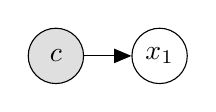
\begin{tikzpicture}
  % Define nodes
  \node[obs]           (c) {$c$};
  \node[latent, right=0.6cm of c]       (x_1) {$x_1$};
  %\node[latent, right=0.6cm of x_1]        (I) {$\mathcal{I}$};

  % Connect the nodes
  \edge {c} {x_1} ; %
  %\edge {x_1} {I} ; %
  %\draw [->] (c) to [out=40,in=140] (I);

\end{tikzpicture}

    %     \caption{A graphical model of the data generating process underlying the proposal distribution $q^*$}
    %     \label{fig:graphical_model}
    % \end{subfigure}
% \end{figure}
% \paragraph{Approximating the Proposal Distribution}
% Even with a closed-form expression for $q^*$, we still do not have an easy way to sample from it. To sample from the posterior $p_{\theta} (x_1|\mathcal{I}=1,c)$, a distribution over high-quality texts, 
\paragraph{E-step}

Maximizing $F(\theta,q)$ w.r.t $q$ corresponds to refining the proposal distribution $q$ to assign higher likelihood to high-quality texts.
%We perform this refinement 
This is achieved by embedding $x_1$ into a data-generating process involving humans, by introducing the initial output $x_0$, and human feedback $f$ (via sum rule):
% and cast $\mathcal{I}$ in terms of human feedback:
\begin{align}
q(x_1|c) &= \sum_{x_0, f} p_{\theta}(x_0, f, x_1|\mathcal{I}=1,c) \label{eq:13}\\
&\propto\sum_{x_0, f}p_{\theta}(x_0,f,x_1|c)p_{\theta}(\mathcal{I}=1|c,x_0, f, x_1) \label{eq:14} \\
&= \sum_{x_0, f} p_{\theta}(x_0|c)p(f|c,x_0)p_{\theta}(x_1|c,x_0,f) \nonumber\\ & \quad\quad\quad p_{\theta}(\mathcal{I}=1|c,x_0, f, x_1).  \label{eq:15}  
\end{align}
%In Eq.~\ref{eq:13}, we introduce latent variables $x_0$, the initial summary, and $f$, the human feedback, using the sum rule. In Eq~\ref{eq:14}, we use Bayes' Rule, and in Eq.~\ref{eq:15}, we factorize the joint distribution $q(x_0,f,x_1)$ using the product rule
Eq. \ref{eq:15} gives rise to the following sampling procedure (see also Fig.~\ref{fig:data_generating_process}, right): First, an LM is conditioned on the context $c$ and generates an initial output $x_0$. Second, a human provides language feedback $f$ on the $(c, x_0)$ pair. Third, the LM generates a refined text $x_1$ conditioned on $(c, x_0, f)$. Finally, a binary variable $\mathcal{I}$ indicates whether $x_1$ is a high-quality text, given an initial output $x_0$, feedback $f$, and a context $c$. We model $p_{\theta}(\mathcal{I}=1|c, x_0, f, x_1)$ as a Boltzmann distribution:
\begin{align}
    p_{\theta}(\mathcal{I}=1|c, x_0, f, x_1) \propto \exp(R(c,x_0,f,x_1)/\beta),\label{eq:boltzmann}
\end{align}
which uses a reward function $R$ defined in terms of four variables: $c, x_0,f,x_1$; $\beta$ is a temperature hyperparameter. This Boltzmann distribution makes quality easy to evaluate since it expresses it as a reward function $R$ of a previous output and human language feedback. 

We now argue why the E-step results in a proposal distribution that is better than the original distribution $p_\theta(x_1|c)$, i.e., why samples from $q(x_1|c)$ tend to be of higher quality than samples from $p_\theta(x_1|c)$. First, we know that $x_0$ is already a reasonably good output (since $\pi_{\theta_\text{old}} \approx \pi_\theta$). We can assume that the feedback $f$ is informative and high-quality. Therefore $x_1 \sim p_\theta(x_1|c,x_0,f)$ is going to be of higher quality than $x_0 \sim p_\theta(x_0|c)$ because it leverages useful information from the feedback.  Furthermore, let us choose $R$ to assign higher values to refined texts $x_1$ that improve upon $x_0$ w.r.t to $f$ and $c$. Consequently, Eq.~\ref{eq:boltzmann} assigns a higher likelihood to high-quality outputs $x_1$, allowing us to put additional weight on high-quality outputs and improving the proposal distribution $q$ further.


% will result in proposal $q(x_1|c)$ being improved over $\pi_\theta(x_1|c)$. 


%\begin{enumerate}
   % \item A LM is conditioned on the document $c$ and generates initial summary $x_0$,
  %  \item A human provides language feedback $f$ on the $(c, x_0)$ pair,
   % \item A LM generates a refined summary $x_1$ conditioned on $(c, x_0, f)$,
   % \item Finally, a binary variable $\mathcal{I}$ indicates whether $x_1$ improves upon $x_0$ with respect to feedback $f$ and source document $c$.
%\end{enumerate}

% This data-generating process gives rise to the following joint distribution:
% \begin{align}
%     q(x_0, f, x_1, \mathcal{I}|c) = &q(x_0|c) q(f|c, x_0)  \\ &q(x_1|f, x_0, c) q(\mathcal{I}|c, x_0, f, x_1) \nonumber
% \end{align}

\paragraph{M-step}

Maximizing $F(\theta,q)$ w.r.t. the policy $\pi_{\theta}$ is equivalent to supervised learning (minimizing cross-entropy loss) on a distribution defined by $q$. To see that, we drop all the terms from Eq.~\ref{eq:four} that do not depend on $\theta$:
\begin{align}
\operatorname*{argmax}_\theta F(\theta, q) 
&= \operatorname*{argmax}_\theta \mathbb{E}_{x_1 \sim q(x_1|c)}  \log p_\theta(x_1,\mathcal{I}=1|c) \nonumber \\
 &= \operatorname*{argmin}_\theta \mathbb{E}_{x_1 \sim q(x_1|c)} -\log \pi_\theta(x_1|c ).\label{eq:supervised_finetuning} \hspace{-10px}
\end{align}
 %In Eq.~\ref{eq:eight} we decompose $\log p_{\theta}(x_1,I=1|c)$, drop $\log p(\mathcal{I}=1|c, x_1)$ as it does not depend on $\theta$ and switch from maximization to minimization.

\paragraph{ILF: Imitation Learning from Language Feedback}
\label{sec:ilf_reward}

In ILF, we alternate between the E-step and M-step, using the pseudocode in Algorithm~\ref{alg:expert_iteration}. In the M-step step, we use the model from the previous iteration $\pi_{\theta_\text{old}}$ as both $p_{\theta}(x_0|c)$ and $p_{\theta}(x_1|c,x_0,f)$. In practice, we implement $R$ by conditioning an instruction-finetuned LM on a binary question such as \textit{Does this new text incorporate the feedback provided? Answer Yes or No.} where the label $y$ is either $y_{\text{good}}$ (`` Yes") or $y_{\text{bad}}$ (`` No"). We use the probability of the positive answer $y_{\text{good}}$ given the prompt as a reward, i.e. $p_\text{norm}(y_{\text{good}}|\text{prompt}) = \frac{p(y_{\text{good}}|\text{prompt})}{p(y_{\text{good}}|\text{prompt}) + p(y_{\text{bad}}|\text{prompt})}$. With these assumptions, $q$ takes the form:
\begin{align*}
   q(x_1|c) \propto &\mathbb{E}_{x_0 \sim \pi_{\theta_\text{old}}(x_0|c)} \mathbb{E}_{f\sim p(f|c,x_0)} \\ &\pi_{\theta_\text{old}}(x_1|c,x_0,f) 
   \exp(R(c,x_0,f,x_1)/\beta).\nonumber
\end{align*}
We take advantage of this proposal distribution and perform the M-step, i.e., $\text{argmax}_{\theta} F(\theta, q)$ on optimized data. 
Finally, we approximate sampling from $q(x_1|c)$ by best-of-$N$ sampling. To obtain a sample $x_1 \sim q$, we %
% first sample $x_0 \sim \pi_{\theta_\text{old}}(x_0|c)$ and $f \sim p(f|c,x_0)$, then
sample $N$ refinements $\{x_1^1, \dots, x_1^N \} \sim \pi_{\theta_\text{old}}(x_1|c,x_0,f)$, and compute
\begin{align*}
x_1 = \text{argmax}_{x_1^i} \exp R(c,x_0, f, x_1^i).
\end{align*}

In summary, we show that ILF can be understood as Bayesian inference. This process involves updating an LM based on the evidence provided by language feedback. This lens highlights the correspondence between ILF and RL with Human Feedback ~\citep[][\textit{inter alia}]{ziegler2019fine, stiennon2020learning}, which was previously demonstrated to be equivalent to Bayesian inference~\citep{korbak2022rl}. 


% from a distribution without the exponential:
% \begin{align*}
% \hat{q}^*(x_1|c) = \mathbb{E}_{x_0 \sim \pi_{\theta_\text{old}}(x_0|c)} \mathbb{E}_{f\sim p(f|c,x_0)} \pi_{\theta_\text{old}}(x_1|c,x_0,f)
% \end{align*}
% using $\exp R(c,x_0,f,x_1)/\beta$ as scores for reranking. 

% In other words, 



% The complete pseudocode is shown in Algorithm~\ref{alg:expert_iteration}. 
%\footnote{To see why approximating sampling from a Boltzmann distribution with best-of-$N$ is justified, note that best-of-all (argmax) corresponds to sampling from $q^*(x_1)$ with temperature to $\beta\to 0$ while best-of-1 (unbiased sampling) corresponds to sampling from  $q^*(x_1)$  with temperature $\beta \to \infty$.} 
%In other words, to obtain a sample $x_1 \sim q^*$, we first sample $x_0 \sim \pi_{\theta_\text{old}}(x_0|c)$ and $f \sim p(f|c,x_0)$, then sample $N$ refinements $\{x_1^1, \dots, x_1^N \} \sim \pi_{\theta_\text{old}}(x_1|c,x_0,f)$, and compute
%\begin{align*}
%x_1 = \text{argmax}_{x_1^i} \exp \frac{1}%{\beta}R(c,x_0, f, x_1^i).
%\end{align*}







%Because we do an EM-style optimization, in the data optimization step we drop the dependence on $\pi_\theta$ and use $\pi_\theta$ from a previous iteration, $\pi_{\theta_\text{old}}$, for both $q(x_0)$ and $q(x_1|x_0,f)$. Additionally, we redefine $q(\mathcal{I}=1|c, x_0, f, x_1)$ as proportional to $\exp(R(c,x_0,f,x_1)/\beta$, a Boltzmann distribution involving a reward function $R$ defined in terms of four variables: $c, x_0,f,x_1$. This is much more tractable in practice because we can now express the notion of quality in terms of a previous summary and human feedback on it: a good summary $x_1$ will improve given feedback $f$ upon $x_0$. Note that that since $\pi_{\theta_\text{old}} \approx \pi_\theta$, we can assume $x_0$ is already pretty good. We also assume that feedback $f$ is informative. Therefore, we can safely assume that improving upon $x_0$ with respect to $f$ corresponds to genuine progress. 
%In practice, we implement $R$ by conditioning an instruction-finetuned LM on a question that elicits a binary answer, such as \textit{Does this new summary incorporate the feedback provided? Answer Yes or No}. The binary label $y$ is either $y_{\text{good}}$ (``Yes") or $y_{\text{bad}}$ (``No"). We then evaluate the normalized probability of $y_{\text{good}
%}$ given the prompt, i.e., $p_\text{norm}(y_{\text{good}}|\text{prompt}) = \frac{p(y_{\text{good}}|\text{prompt})}{p(y_{\text{good}}|\text{prompt}) + p(y_{\text{bad}}|\text{prompt})}$, and use this normalized probability as a reward. 


%(such as \textit{Yes} or \textit{No}) and use the log-likelihood of the corresponding tokens as a reward. In the case of summarization, the question could, for example, be \textit{Does the following refinement include the feedback on the initial summary?}. We call this reward model \textit{InstructRM}.

% In practice, we implement $R$ by




We present in section~\ref{ssec:faces} an application of PnP-HVAE on face images, using a pretrained state-of-the-art hierarchical VAE. 
Next, we study the application of our framework to natural images. To that end, we introduce  in section~\ref{ssec:patchVDVAE}  a patch hierachical VAE architecture, that is able to model natural images of different resolutions. In section~\ref{ssec:app_nat}, we provide deblurring, super-resolution and inpainting experiments to demonstrate the relevance of the proposed method.

Additional results are presented in Appendix~\ref{app:add}. All experiments can be reproduced using the code available at \url{https://github.com/jprost76/PnP-HVAE}.



\subsection{Face Image restoration (FFHQ)}\label{ssec:faces}
We first demonstrate the effectiveness of PnP-HVAE on highly structured data, by performing face image restoration.
Latent variable generative models can accurately model structured images such as face images \cite{karras2019style,vahdat2020nvae,child2021very,kingma2018glow}, and then be used to produce high quality restoration of such data. 
In our experiments, we use the VDVAE model of~\cite{child2021very}, pre-trained on the FFHQ dataset~\cite{karras2019style}, as our hierarchical VAE prior.
VDVAE has $L=66$ latent variable groups in its hierarchy and generates images at resolution $256\times256$.

We compare PnP-HVAE with the intermediate layer optimization algorithm (ILO)~\cite{daras2021intermediate} that is based on a different class of generative models than HVAE. ILO is a GAN inversion method which optimizes the image latent code along with the intermediate layer representation of a StyleGAN to generate an image consistent with a degraded observation.
We use the official implementation of ILO, along with a StyleGAN2 model~\cite{karras2020analyzing, stylegan2pytorch}, that was trained for 550k iterations on images of resolution $256\times256$ from FFHQ.  
As VDVAE and StyleGAN models are not trained on the same train-test split of FFHQ, we chose to evaluate the methods on a subset of 100 images from the CelebA dataset~\cite{liu2018large}. 
For super-resolution, the degradation model corresponds to the application of a gaussian low-pass filter followed by a $\times 4$ sub-sampling, and the addition of a gaussian white noise with $\sigma=3$.
For the deblurring, we considered motion blur and  gaussian kernels, both with a noise level $\sigma=8$. %

We provide quantitative comparisons in table~\ref{table:comp_ILO}, along with a visual comparison of the results in figure~\ref{fig:face_restoration}.
PnP-HVAE has the best  PSNR and SSIM results for all the considered restoration tasks, while ILO provides better results  for the perceptual distance.
By jointly optimizing the image and its latent variable, PnP-HVAE provides  results that are both realistic and consistent with the degraded observation.
On the other hand,  ILO  only optimizes on an extended latent space. This method generates  sharp and realistic images with better LPIPS scores,   
but the results lack  of consistency with respect to the observation, which explains the overall lower PSNR performance. 






\subsection{PatchVDVAE: a HVAE for natural images}\label{ssec:patchVDVAE}
Available generative models in the literature operate on images of  fixed resolutions and
are either restrained to datasets of limited diversity, or even to registered face images~\cite{kingma2018glow,child2021very, vahdat2020nvae, karras2019style}, or requiring additional class information~\cite{brock2018large, dhariwal2021diffusion, song2020score, luhman2022optimizing}.
Fitting an unconditional model on natural images appears to be a more difficult task, as their resolution can change, and their content is highly diverse.
The complexity of the problem can be reduced by learning a prior model on patches of reduced dimension. 
For image restoration problems, the patch model can be reused on images of higher dimensions~\cite{zoran2011learning,prost2021learning,altekruger2022patchnr}. When the model is a full CNN, the prior on the set of the  patches can  be computed efficiently by applying the network on the full image~\cite{prost2021learning}.

We thus introduce  patchVDVAE, a fully convolutional hierarchical VAE.
Contrary to existing HVAE models whose resolution is constrained by the constant tensor at the input of the top-down block, patchVDVAE can generate images of different resolutions by controlling the dimension of the input latent. 
This amounts to defining a prior on patches whose dimension corresponds to the receptive field of the VAE. A similar model is used for image denoising in~\cite{prakash2021interpretable}.

 
For PatchVDVAE architecture, we use the same bottom-up and top-down blocks as VDVAE~\cite{child2021very}, and replace the constant trainable input in the first top-down block by a latent variable, to make the model fully convolutional (details on the  architecture are given in Appendix~\ref{app:details}). 
The training dataset is composed of $128\times 128$ patches extracted from a combination of DIV2K~\cite{agustsson2017ntire} and Flickr2K~\cite{Lim_2017_CVPR_workshops} datasets.
We perform data augmentation by extracting  patches at $3$ resolutions: HR-images and $\times 2$ and $\times 4$ downscaled images. 
The model is trained for $7.10^5$ iterations with a batch size of $64$. Following the recommendation of~\cite{hazami2022efficient}, we use Adamax optimizer with an exponential moving average and gradient smoothing of the variance.
We set the decoder model to be a gaussian with diagonal covariance, as in~\cite{luhman2022optimizing}.
PatchVDVAE is fully convolutional and can generate images of dimension that are multiples of $64$ as illustrated by
figure~\ref{fig:vdvae}.

\newlength{\patchwidth}
\setlength{\patchwidth}{0.135\columnwidth}
\begin{figure}[!ht]
    \centering
    \begin{subfigure}[t]{.34\columnwidth}\hspace{0.1cm}
        \setlength{\tabcolsep}{0.02pt}
\renewcommand{\arraystretch}{0}
        \begin{tabular}{*{2}{p{1.03\patchwidth}}}
            \includegraphics[width=\patchwidth]{figures_arxiv/patchVDVAE/samples/generated/64x64/setup-5-image-0018.png} &
            \includegraphics[width=\patchwidth]{figures_arxiv/patchVDVAE/samples/generated/64x64/setup-5-image-0016.png} \\
            \includegraphics[width=\patchwidth]{figures_arxiv/patchVDVAE/samples/generated/64x64/setup-5-image-0008.png} &
            \includegraphics[width=\patchwidth]{figures_arxiv/patchVDVAE/samples/generated/64x64/setup-5-image-0019.png}   
        \end{tabular}
    \end{subfigure}\hspace{-0.15cm}
    \begin{subfigure}[t]{.64\columnwidth}
\begin{tabular}{cc}\vspace{-0.1cm}
\includegraphics[width=2\patchwidth]{figures_arxiv/patchVDVAE/samples/generated/256x256/setup-2-image-0009.png}&
        \includegraphics[width=2\patchwidth]{figures_arxiv/patchVDVAE/samples/generated/256x256/setup-2-image-0002.png}\end{tabular}

    \end{subfigure}
    \caption{\label{fig:vdvae} Left: $64\times64$ patches samples from our patchVDVAE model trained on patches from natural images.
    Right: PatchVDVAE is fully convolutional and it can generate images of higher resolution (here: $128\times128$).\vspace{-0.2cm}}
\end{figure}

\subsection{Natural images restoration}\label{ssec:app_nat}
We  evaluate PnP-HVAE on natural image restoration.
For each task, we report the average value of the PSNR, the SSIM, and the LPIPS metrics on $20$ images from the test set of the BSD dataset~\cite{MartinFTM01}.\\


\noindent
{\bf Image deblurring.}
In the experiments, we consider $2$ gaussian kernels and $2$ motion blur kernels from~\cite{levin2009understanding}, with $3$ different noise levels 
$\sigma \in \{2.55, 7.65, 12.75\}$.
As a baseline we consider  EPLL~\cite{zoran2011learning}, which learns a prior on image patches with a gaussian mixture model.
We also compare PnP-HVAE  with PnP-MMO and GS-PnP, $2$ competing convergent Plug-and-Play methods based on CNN denoisers.
PnP-MMO~\cite{pesquet2021learning} restricts the denoiser to be contraction in order to guarantee the convergence of the PnP forward-backard algorithm. GS-PnP~\cite{hurault2022gradient} considers a gradient step denoiser and reaches state-of-the-art performances of non converging methods~\cite{zhang2021plug}.
We set the temperature $\tau$  in our method as $0.95$, $0.8$ and $0.6$ for noise levels $2.55$, $7.65$ and $12.75$ respectively, and we let it run for a maximum of $50$ iterations. 
For the three compared methods we use the official implementations and pre-trained models provided by the respective authors. 
Details on the choice of hyperparameters for the concurrent methods are provided in the Appendix~\ref{app:details}
Figure~\ref{fig:deblurring_bsd} illustrates that our method provides correct deblurring results. 

According to table~\ref{tab:deb}, the performance of PnP-HVAE is between those of EPLL and GS-PnP and it outperforms PnP-MMO for large noise levels.\\

\begin{table}
\begin{center}\footnotesize
    \begin{tabular}{>{\centering}m{.3cm}*{5}{c}}
    $\sigma$ &Method & PSNR$\uparrow$ & SSIM$\uparrow$ & LPIPS$\downarrow$  \\ 
    \hline
    \multirow{4}{*}{\vcell{$2.55$}}
    & PnP-HVAE & $27.75$ & $0.79$ & $0.31$\\
    & GS-PNP \cite{hurault2022gradient} & $\mathbf{29.59}$ & $\mathbf{0.84}$ & $\mathbf{0.22}$\\
    & EPLL \cite{zoran2011learning} & $26.49$ & $0.71$ & $0.36$\\ 
    & PnP-MMO \cite{pesquet2021learning} & $\underbar{29.50}$ & $\underbar{0.83}$ & $\underbar{0.20}$ \\ \hline
    \multirow{4}{*}{\vcell{$7.65$}}
    & PnP-HVAE & $\underbar{26.36}$ & $\underbar{0.72}$ & $\underbar{0.40}$\\
    & GS-PNP \cite{hurault2022gradient} & $\mathbf{27.33}$ & $\mathbf{0.77}$ & $\mathbf{0.31}$\\
    & EPLL \cite{zoran2011learning} & $24.04$ & $0.66$ & $0.45$ \\ 
    & PnP-MMO \cite{pesquet2021learning} & $25.34$ & $0.69$ & $0.34$\\
    \hline
    \multirow{4}{*}{\vcell{$12.75$}}
    & PnP-HVAE & $\underbar{25.12}$ & $\mathbf{0.73}$ & $\underbar{0.47}$\\
    & GS-PNP \cite{hurault2022gradient} & $\mathbf{26.32}$ & $\mathbf{0.73}$ & $\mathbf{0.37}$\\
    & EPLL \cite{zoran2011learning} & $23.28$ & $0.61$ & $0.51$ \\ 
    & PnP-MMO \cite{pesquet2021learning} & $22.42$ & $0.53$& $0.54$ \\
    \hline
    &\vspace*{-.3cm}\\
            \multicolumn{2}{c}{Blur and motion kernels}& \multicolumn{3}{c}{
        \includegraphics*[scale=1]{figures_arxiv/kernels/4.png}\;\includegraphics*[scale=1]{figures_arxiv/kernels/7.png}\;\includegraphics*[scale=1]{figures_arxiv/kernels/9.png}\;\includegraphics*[scale=1]{figures_arxiv/kernels/11.png}} 
    \end{tabular}
        \caption{\label{tab:deb}Comparison  of PnP-HVAE  and other restoration methods on deblurring. Results are averaged on $4$ kernels.\vspace{-0.2cm}}% on image deblurring.}
    \end{center}
\end{table}

\begin{figure}
    
    \begin{subfigure}[h]{\linewidth}
        \centering
        \includegraphics*[width=\columnwidth]{figures_arxiv/deb_s255_k7.pdf}\vspace{-0.1cm}
        \caption{Gaussian blur, $\sigma=2.55$}
    \end{subfigure}
    \begin{subfigure}[h]{\linewidth}
        \centering
        \includegraphics*[width=\columnwidth]{figures_arxiv/deb_s765_k11.pdf}\vspace{-0.1cm}
        \caption{Motion blur, $\sigma=7.65$}
    \end{subfigure}\vspace*{-0.1cm}
    \caption{\label{fig:deblurring_bsd} Natural image deblurring\vspace{-0.1cm}}
\end{figure}

\noindent {\bf Effect of the temperature.}
PnP-HVAE gives control on the temperature of the prior over the latent space.
In figure~\ref{fig:temp_effect}, we illustrate that reducing the temperature increases the strength of the regularization prior. In this example the tuning $\tau=0.7$ produces the best performance.\\
\begin{figure}[!ht]
   
    \includegraphics[width=\columnwidth]{figures_arxiv/demo_temp.pdf}\vspace{-0.15cm}
    \caption{ \label{fig:temp_effect} Effect of the temperature in PnP-VAE on a deblurring problem, with $\sigma=7.65$.\vspace{-0.15cm}}
\end{figure}


\noindent
{\bf Image inpainting.}
Next we consider the task of noisy image inpainting. 
We compose a test-set of 10 images from the validation set of BSD~\cite{MartinFTM01} and we create masks
  by occluding diverse objects of small size in the images. 
A gaussian white noise with $\sigma=3$ is added to the images.
As a comparaison, we still consider GS-PnP and EPLL.
For PnP-HVAE, the temperature is set to $\tau=0.6$, and the algorithm is run for a maximum of $200$ iterations, unless the residual $||\x_{k+1}-\x_k||$ is on a plateau.
We provide on Table~\ref{tab:inpainting_bsd} the distortion metrics with the ground truth, as well as a visual
\begin{table}



\begin{center}
    \begin{tabular}{cccc}
        & PSNR$\uparrow$ & SSIM$\uparrow$ &LPIPS$\downarrow$ \\\hline
        PnP-HVAE  & $\mathbf{29.54}$ & $\mathbf{0.93}$ & $\mathbf{0.06}$\\
        GS-PNP & $28.52$ & $\mathbf{0.93}$ & $0.09$\\
        EPLL & $\underline{29.16}$ & $\mathbf{0.93}$ & $\mathbf{0.06}$\\
    \end{tabular}
    \caption{\label{tab:inpainting_bsd}Quantitative evaluation for inpainting on BSD.}
    \end{center}
\end{table}
comparison on figure~\ref{fig:inpainting_bsd}. 
With its hierarchical structure,  PnP-HVAE outperforms the compared methods. \vspace{0.05cm}



\begin{figure}[!h]
    \includegraphics[width=\columnwidth]{figures_arxiv/demo_inp_bsd2.pdf}\vspace{-0.1cm}
    \caption{\label{fig:inpainting_bsd}Natural image inpainting\vspace{-0.3cm}}
\end{figure}











\section{Related work}
% There is extensive recent work on speeding up analytical queries due to the need for consistent execution times in the face of the explosive growth in the volume of available data.
% In this section, we divide existing work into two categories: maintaining data freshness in MVs (\Cref{sec:server_side}) and optimizations for minimizing ad-hoc query latency (\Cref{sec:client_side}).

% \subsection{Maintaining Data Freshness in MVs}
% \label{sec:server_side}
% There exists a variety of data warehousing applications aimed at supporting low-latency analytical queries on fresh data.
% In particular, these applications require efficiency in the propagation of newly ingested data into downstream MVs.
 
\mypara{Efficient MV Refresh}
Incremental view maintenance (IVM) aims to update MVs to reflect newly ingested data, taking advantage of already computed results to perform the update in a manner more efficient than computing from scratch (full refresh)
~\cite{ahmad2012dbtoaster,mcsherry2013differential,armbrust2013generalized,zeng2016iolap, palpanas2002incremental, griffin1995incremental, agiwal2021napa, braun2015analytics}. 
There is an abundance of work in IVM, including incremental updates on duplicate values~\cite{griffin1995incremental}, non-distributive aggregate functions~\cite{palpanas2002incremental}, higher-order views~\cite{ahmad2012dbtoaster}, and sliding windows~\cite{braun2015analytics}. 
More recent works also investigate the scalability aspect of IVM, proposing scale-independent updates~\cite{armbrust2013generalized} and sampled views~\cite{zeng2016iolap}. Since \system is applicable to arbitrary SQL statements, \system is orthogonal to and is fully compatible with existing IVM techniques.

\mypara{MV Refresh Scheduling}
There exist works on scheduling the refresh of a MV set focusing on resolving cyclic dependencies~\cite{folkert2005optimizing}, minimizing weighted average staleness~\cite{golab2009scheduling}, and prioritizing MVs with the highest speedups on predicted future queries~\cite{ahmed2020automated}.
\system's scheduling to speed up the end-to-end refresh of the MV set is not addressed in existing works.

\mypara{DAG Workflow Scheduling}
The execution of workloads consisting of individual jobs with acyclic dependencies is a well-studied topic~\cite{apacheoozie,sparkdag,marchal2018parallel,bathie2020revisiting,baruah2022ilp}; many of these techniques can be applied to MV refresh runs studied in this paper.
Existing workflow scheduling systems such as Apache Oozie~\cite{apacheoozie}, Apache Airflow~\cite{airflow}, and Spark DAG scheduler~\cite{sparkdag} automate the execution of user-defined workflows following a topological order.
There are recent works aimed at finding more optimal execution orders in terms of peak memory usage~\cite{marchal2018parallel, bathie2020revisiting} and execution time on parallel platforms~\cite{baruah2022ilp}.
While \system is designed for use with MV refresh runs/workloads, our technique on joint scheduling and optimization can be reasonably applied to general workloads as a possible future direction.

% \paragraph{Incremental MV indexing}
% Update-optimized indices such as the log-structured merge-trees (LSM)~\cite{o1996log} are used for indexing MVs due to frequent updates induced by data ingestion~\cite{gupta2016mesa,agiwal2021napa}.
% \system is orthogonal to indexing: \system is capable of efficiently performing MV refresh runs regardless of whether the individual MVs are indexed or not.

% \subsection{Ad-hoc Query Latency Reduction}
% \label{sec:client_side}

% The minimization of ad-hoc analytical query response times is a well-studied topic due to latency being negatively correlated with the productivity of a data analyst during a data analysis session~\cite{liu2014effects}.
% Sessions are commonly conducted within visualization systems that contain a variety of optimization techniques to ensure that query response times fall within a certain latency tolerance.

% \mypara{Data prefetching}
% Data is often loaded into memory on a by-need basis in visualization systems to minimize interference with user-issued query computations~\cite{mani2017effective,xin2021enhancing,galakatos2017revisiting, yan2020auto, battle2016dynamic, crotty2016case, jalaparti2018netco}. 
% Query-time data retrieval can be significantly expedited by anticipating the data usage of the user in future queries and pre-loading the data into memory during the downtime between user queries (`think time'). SMART~\cite{mani2017effective} prefetches data for modified versions of current user-issued queries with different filters and dimensions. A-WARE~\cite{crotty2016case} maintains a sample store constantly refined through ingesting data based on speculations of future plots.
% ForeCache~\cite{battle2016dynamic} uses an SVM to predict the user's current analysis phase and accordingly prefetches data tiles partitioned based on different numerical values. NetCo predicts future queries via log analysis, and solves an ILP formulation to prefetch data to maximize the number of SLO-meeting queries~\cite{jalaparti2018netco}.
% In the case of MV refresh workloads, `think time' is nonexistent as individual MVs are refreshed back-to-back, rendering data prefetching techniques non-applicable.

\mypara{Intermediate Data Caching}
Some existing data visualization systems cache user-defined variables to support the typical incremental construction of data visualizations~\cite{zgraggen2016progressive, eichmann2020idebench} during data analysis sessions~\cite{jupyter, rstudio, colab}. 
Recent work proposes a management scheme for these cached variables under a memory constraint that greedily keeps variables with the highest estimated time savings based on predicted future user behavior via neural networks~\cite{xin2021enhancing}.
While useful for data visualization, a greedy approach to memory management fails to achieve satisfactory results compared to \system.

\mypara{Intermediate Result Reuse}

There exist works on storing intermediate results from computations to speedup future computations~\cite{yang2018intermediate, dursun2017revisiting, nagel2013recycling, michiardi2019memory, galakatos2017revisiting}.
Studied topics include the identification of reuse opportunities by finding overlaps in computation graphs of successive jobs~\cite{yang2018intermediate, michiardi2019memory},
selective storage under a space constraint with heuristics such as reuse probability~\cite{dursun2017revisiting}, expected savings~\cite{yang2018intermediate}, and recompute-storage cost difference~\cite{nagel2013recycling},
and rewriting incoming jobs to take advantage of stored intermediates~\cite{galakatos2017revisiting}.
These works share similarity with \system in their selection of items to store under a memory constraint, however, \system's problem setting requires it to uniquely consider the joint (re)ordering of job executions along with the selection of items.

% work that considers both job execution (re)order as well as intermediate result caching with a bounded amount of memory. but notably lack the joint aspect of \system and cannot be used to achieve immediate speedup on an incoming MV refresh run if no intermediates are stored beforehand. 

\mypara{Incremental Query Processing} Incremental processing (IQP) is useful for cases where not all data required for a query is immediately available. Similar to online aggregation~\cite{hellerstein1997online}, initial results of a query are computed on a subset of required data and progressively refined as the rest of the required data arrives in a predictable pattern~\cite{tang2019intermittent,wangtempura}. Tang et al. propose a dynamic programming formulation to pick intermediate states to store in memory given a limited memory budget~\cite{tang2019intermittent}. Tempura rewrites the query plan for more efficient execution based on predicted data arrival patterns~\cite{wangtempura}. While similarities exist between the problem setting of IQP and \system, such as management of bounded memory, \system notably includes additional joint optimization for the order of MV updates.

% \paragraph{Sampling}
% Sampling has seen wide use in visualization systems for reducing the computation time of ad-hoc queries by computing an approximate result over a subset of data as exact results are not always required by the user~\cite{crotty2016case, mani2017effective, zgraggen2014panoramicdata, kraska2021northstar, galakatos2017revisiting, kandula2016quickr}. 
% Commonly studied topics in sampling for ad-hoc queries include complex query sampling~\cite{kandula2016quickr}, rare event aggregation~\cite{kraska2021northstar, galakatos2017revisiting}, and maintaining consistency between related sampled visualizations~\cite{zgraggen2014panoramicdata}.
% Sampling server-side at the MV level compromises the assumptions of downstream applications and is thus not considered in \system.

% \paragraph{Progressive visualization}
% The latency tolerance for time-consuming queries can be circumvented by presenting a partially-computed visualization to the user within the tolerance, which is then incrementally refined until it is fully accurate~\cite{rahman2017ve, zgraggen2016progressive, crotty2015vizdom, kraska2021northstar, kamat2017infiniviz}.
% Example plots which benefit from progressive visualization include bar charts~\cite{kamat2017infiniviz} and heatmaps~\cite{rahman2017ve}.
% Similar to sampling, study on this topic is orthogonal to \system as pushing out partially-updated MVs compromises downstream assumptions.
\section{Conclusion}\label{sec:conclusion}
In this work, we focus on addressing the fundamental challenge of OOD detection tasks, which is how to fully understand the semantic discrepancy between the ID/OOD samples. We reveal that the key to success in the realistic SCOOD task is to allocate as many ID samples in the unlabeled set correctly as possible. To this end, we propose a novel uncertainty-aware optimal transport scheme that introduces class-specific energy scores as guidance for effective label assignment. Experimental results show that our method achieves better performance than previous state-of-the-art methods on SCOOD benchmarks.

\textbf{Limitations.} In addition to temperature scaling, other techniques such as feature clipping applied in ReAct~\cite{sun2021react} also enhance the performance of energy score, so how to obtain an OOD score that best fits the SCOOD task can be further explored. Moreover, a setting highly related to SCOOD has been proposed in \cite{katz2022training} and formulated as a constrained optimization problem. We will also theoretically analyze these practical OOD settings in our feature work.

% \section*{Acknowledgments}
\textbf{Acknowledgments.} 
This work is supported by National Key R\&D Program of China under Grant 2020AAA0105701, National Natural Science Foundation of China (NSFC) under Grants 61872327, Major Special Science and Technology Project of Anhui, National Natural Science Foundation of China (62033012) and Ant Group through Ant Research Intern Program.

\chapter*{Acknowledgement}
\addcontentsline{toc}{chapter}{Acknowledgement}
The authors thank Andrzej Kupsc, Sergey Barsuk, Olivier Callot and Wolfgang K{\"u}hn for their contribution on the CDR draft.
%The authors thank the international review committee XXX for their great effort in reading the CDR draft and providing valuable suggestions. 
The STCF working group thanks all 
the colleagues in the world-wide community for many profitable discussions
and expresses gratitude to the Hefei Comprehensive National Science Center for their strong support.  This work is supported by: international 
partnership program of the Chinese Academy of Sciences Grant No. 211134KYSB20200057.

\bibliography{references}
\bibliographystyle{icml2023}


%%%%%%%%%%%%%%%%%%%%%%%%%%%%%%%%%%%%%%%%%%%%%%%%%%%%%%%%%%%%%%%%%%%%%%%%%%%%%%%
%%%%%%%%%%%%%%%%%%%%%%%%%%%%%%%%%%%%%%%%%%%%%%%%%%%%%%%%%%%%%%%%%%%%%%%%%%%%%%%
% APPENDIX
%%%%%%%%%%%%%%%%%%%%%%%%%%%%%%%%%%%%%%%%%%%%%%%%%%%%%%%%%%%%%%%%%%%%%%%%%%%%%%%
%%%%%%%%%%%%%%%%%%%%%%%%%%%%%%%%%%%%%%%%%%%%%%%%%%%%%%%%%%%%%%%%%%%%%%%%%%%%%%%
\newpage

\appendix
\onecolumn
\section{Appendix for Proofs}

\paragraph{Proof of Theorem \ref{thm:main}.}

\begin{proof}
\label{proof:main}
Our proof has two steps. In Step 1, we will show that SimCLR is equivalent to minimizing the cross entropy loss defined in Eqn.~(\ref{eqn:cross-entropy}). 
In Step 2, we will show  that minimizing the cross-entropy loss 
is equivalent to spectral clustering on $\bfpi$. 
Combining the two steps together, we have proved our theorem. 

\textbf{Step 1: } SimCLR is equivalent to minimizing the cross entropy loss.

The cross-entropy loss takes expectation over 
$\bfW_\bfX\sim \mathbb{P}(\cdot ; \bfpi)$, 
which means $\bfW_\bfX$ has exactly one non-zero entry in each row $i$. By Lemma~\ref{lem:multinomial}, we know every row $i$ of $\bfW_\bfX$ is independent of other rows. Moreover, 
$\bfW_{\bfX,i}\sim \mathcal{M}(1, \bfpi_i/\sum_j \bfpi_{i,j})=\mathcal{M}(1, \bfpi_i)$, because $\bfpi_i$ itself is a probability distribution.
Similarly, we know $\bfW_\bfZ$ also has the row-independent property by sampling over $\mathbb{P}(\cdot;\bfK_\bfZ)$.
Therefore, by Lemma~\ref{lem:cross_split}, we know Eqn.~(\ref{eqn:cross-entropy}) is equivalent to:
\[
 -\sum_{i=1}^n \mathbb{E}_{\bfW_{\bfX,i}}[\log \mathbb{P}(\bfW_{\bfZ,i}=\bfW_{\bfX,i};\bfK_\bfZ)],
\]

This expression takes expectation over $\bfW_{\bfX,i}$ for the given row $i$. Notice that 
$\bfW_{\bfX,i}$ has exactly one non-zero entry, which equals $1$ (same for $\bfW_{\bfZ,i}$). 
As a result
we expand the above expression to be:
\begin{equation}
 -\sum_{i=1}^n \sum_{j\neq i} \Pr(\bfW_{\bfX,i,j}=1)\log \Pr(\bfW_{\bfZ,i,j}=1).
\label{eqn:detailed-expansion}    
\end{equation}


By Lemma~\ref{lem:multinomial}, $\Pr(\bfW_{\bfZ,i,j}=1)=\bfK_{\bfZ,i,j}/\|\bfK_{\bfZ,i}\|_1$ for $j\neq i$. Recall that $\bfK_\bfZ=(k(\bfZ_i-\bfZ_j))_{(i,j)\in[n]^2}$, which means 
$\bfK_{\bfZ,i,j}/\|\bfK_{\bfZ,i}\|_1=\frac{\exp(-\|\bfZ_i-\bfZ_j\|^2/{2\tau})}{\sum_{k\neq i}
\exp(-\|\bfZ_i-\bfZ_k\|^2/{2\tau})
}$ for $j\neq i$, when $k$ is the Gaussian kernel with variance $\tau$. 

Notice that $\bfZ_i=f(\bfX_i)$, so we know
\begin{equation}
-\log \Pr(\bfW_{\bfZ,i,j}=1)=
-\log \frac{\exp(-\|f(\bfX_i)-f(\bfX_j)\|^2/{2\tau})}{\sum_{k\neq i}
\exp(-\|f(\bfX_i)-f(\bfX_k)\|^2/{2\tau}),
}
\label{eqn:infonce-equivalence}    
\end{equation}


The right hand side is exactly the InfoNCE loss defined in Eqn.~(\ref{eqn:infonce}).
Inserting Eqn.~(\ref{eqn:infonce-equivalence}) into Eqn.~(\ref{eqn:detailed-expansion}), we get the SimCLR algorithm, which first samples augmentation pairs $(i,j)$ with $\Pr(\bfW_{\bfX,i,j}=1)$ for each row $i$, and then optimize the InfoNCE loss. 

\textbf{Step 2: } minimizing the cross entropy loss 
is equivalent to spectral clustering on $\bfpi$.


By Lemma~\ref{lem:convert_to_spectral}, we may further convert the loss to 
\begin{equation}
\label{eqn:main-theorem-repul-attr}
\min_{\bfZ}
-\sum_{(i,j)\in [n]^2} \mathbf{P}_{i,j}
\log k (\bfZ_i-\bfZ_j)+\log \mathbf{R}(\bfZ).
\end{equation}
Since $k$ is the Gaussian kernel, this reduces to \[
\min_\bfZ \mathrm{tr}(\bfZ^\top \mathbf{L}(\bfpi) \bfZ)
+\log \mathbf{R}(\bfZ),
\]

where we use the fact that $\mathbb{E}_{\bfW_\bfX\sim \mathbb{P}(\cdot; \bfpi)}[\mathbf{L}(\bfW_\bfX)]
=\mathbf{L}(\bfpi)
$, because the Laplacian operator is linear and $
\mathbb{E}_{\bfW_\bfX\sim \mathbb{P}(\cdot; \bfpi)}(\bfW_\bfX)=\bfpi
$.
\end{proof}

\paragraph{Proof of Theorem \ref{thm:clip}.}
\begin{proof}
Since $\bfW_\bfX\sim \mathbb{P}(\cdot;\bfpi_{\mathbf{A}, \mathbf{B}})$, we know 
$\bfW_\bfX$ has exactly one non-zero entry in each row, denoting the pair that got sampled. 
A notable difference compared to the previous proof is we now have $n_\mathcal{A}+n_\mathcal{B}$ objects in our graph. CLIP deals with this by taking a mini-batch of size $2N$, 
such that $n_\mathcal{A}=n_\mathcal{B}=N$, and adding the $2N$ InfoNCE losses together. We label the objects in $\mathcal{A}$ as $[n_\mathcal{A}]$, and the objects in $\mathcal{B}$ as $\{n_\mathcal{A}+1, \cdots, n_\mathcal{A}+n_\mathcal{B}\}$. 

Notice that $\bfpi_{\mathbf{A}, \mathbf{B}}$ is a bipartite graph, so the edges of objects in $\mathcal{A}$ will only connect to object in $\mathcal{B}$ and vice versa. We can define the similarity matrix in $\cZ$ as $\bfK_\bfZ$, 
where $\bfK_\bfZ(i, j+n_\mathcal{A})=\bfK_\bfZ(j+n_\mathcal{A},i)= k(\bfZ_i-\bfZ_j)$ for $i\in [n_\mathcal{A}], j\in [n_\mathcal{B}]$, and otherwise we set $\bfK_\bfZ(i,j)=0$. 
The rest is same as the previous proof. 
\end{proof}

\paragraph{Proof of Theorem \ref{thm:exponential}.}

\begin{proof}
\label{proof:exponential}
Since the objective function consists of a linear term combined with an entropy regularization, which is a strongly concave function, the maximization problem is a convex optimization problem. Owing to the implicit constraints provided by the entropy function, the problem is equivalent to having only the equality constraint. We then introduce the Lagrangian multiplier $\lambda$ and obtain the following relaxed problem:

$$
\widetilde{E}(\boldsymbol{\alpha})=\psi_{1}-\sum_{i=1}^n \alpha_{i} \psi_{i}+\tau \sum_{i=1}^n \alpha_{i}\log \alpha_{i}+\lambda\left(\boldsymbol{\alpha}^{\top} \mathbf{1}_n-1\right).
$$

As the relaxed problem is unconstrained, taking the derivative with respect to $\alpha_{i}$ yields

$$
\frac{\partial \widetilde{E}(\boldsymbol{\alpha})}{\partial \alpha_{i}}=-\psi_{i}+\tau\left(\log \alpha_{i}+\alpha_{i} \frac{1}{\alpha_{i}}\right)+\lambda=0.
$$

Solving the above equation implies that $\alpha_{i}$ takes the form
$
\alpha_{i}=\exp \left(\frac{1}{\tau} \psi_{i}\right) \exp \left(\frac{-\lambda}{\tau}-1\right).
$ Since $\alpha_{i}$ lies on the probability simplex, the optimal $\alpha_{i}$ is explicitly given by
$
\alpha^{*}_{i}=\frac{\exp \left(\frac{1}{\tau} \psi_{i}\right)}{\sum_{i^{\prime}=1}^n \exp \left(\frac{1}{\tau} \psi_{i^{\prime}}\right)} .
$ Substituting the optimal point into the objective function, we obtain
$$
\begin{aligned}
E\left(\boldsymbol{\alpha}^*\right)  &=\psi_1-\sum_{i=1}^n \frac{\exp \left(\frac{1}{\tau} \psi_{i}\right)}{\sum_{i^{\prime}=1}^n \exp \left(\frac{1}{\tau} \psi_{i^{\prime}}\right)} \psi_{i}+\tau \sum_{i=1}^n \frac{\exp \left(\frac{1}{\tau} \psi_{i}\right)}{\sum_{i^{\prime}=1}^n \exp \left(\frac{1}{\tau} \psi_{i^{\prime}}\right)}\log \frac{\exp \left(\frac{1}{\tau} \psi_{i}\right)}{\sum_{i^{\prime}=1}^n \exp \left(\frac{1}{\tau} \psi_{i^{\prime}}\right)} \\
& =\psi_1 - \tau \log \left(\sum_{i=1}^n \exp \left(\frac{1}{\tau} \psi_{i}\right)\right).
\end{aligned}
$$
Thus, the Lagrangian dual function is given by
\begin{equation*}
-E\left(\boldsymbol{\alpha}^*\right)= -\tau \log \frac{\exp \left(\frac{1}{\tau} \psi_{1}\right)}{\sum_{i=1}^n \exp \left(\frac{1}{\tau} \psi_{i}\right)}.\qedhere
\end{equation*}
\end{proof}



\section{More on Experiments} \label{section: experiment_details}

\paragraph{CIFAR-10 and CIFAR-100} CIFAR-10 ~\citep{krizhevsky2009learning} and CIFAR-100 ~\citep{krizhevsky2009learning} are well-known classic image classification datasets. Both CIFAR-10 and CIFAR-100 contain a total of 60k $32 \times 32$ labeled images of different classes, with 50k for training and 10k for testing. CIFAR-10 is similar to CIFAR-100, except there are 10 different classes in CIFAR-10 and 100 classes in CIFAR-100.

\paragraph{TinyImageNet} TinyImageNet ~\citep{le2015tiny} is a subset of ImageNet ~\citep{deng2009imagenet}. There are 200 different object classes in TinyImageNet, with 500 training images, 50 validation images, and 50 test images for each class. All the images in TinyImageNet are colored and labeled with a size of $64 \times 64$.

\textbf{Pseudo-code.} Algorithm \ref{alg:Training Procedure} presents the pseudo-code for our empirical training procedure.

\begin{algorithm}[!htbp]
\caption{Training Procedure}
\label{alg:Training Procedure}
\begin{algorithmic}[1]
\REQUIRE trainable encoder network $f$, batch size $N$, augmentation strategy \textit{aug}, loss function $L$ with hyperparameters \textit{args}
\FOR {sampled minibatch ${x_i}_{i=1}^N$}
\FORALL{$i \in { 1, ..., N }$}
\STATE draw two augmentations $t_i = \textit{aug}\left(x_i\right) $, $t_i' = \textit{aug}\left(x_i\right) $
\STATE $z_i = f\left(t_i\right)$, $z_i' = f\left(t_i'\right)$
\ENDFOR
\STATE compute loss $\mathcal{L} = L(N, z, z', \textit{args})$
\STATE update encoder network $f$ to minimize $\mathcal{L}$
\ENDFOR
\STATE \textbf{Return} encoder network $f$
\end{algorithmic}
\end{algorithm}

We also provide the pseudo-code for our core loss function used in the training procedure in Algorithm \ref{alg:Core loss}. The pseudo-code is almost identical to SimCLR's loss function, with the exception of an extra parameter $\gamma$.

\begin{algorithm}[!htbp]
\caption{Core loss function $\mathcal{C}$}
\label{alg:Core loss}
\begin{algorithmic}[1]
\REQUIRE batch size $N$, two encoded minibatches $z_1, z_2$, $\gamma$, temperature $\tau$
\STATE $z = \textit{concat}\left(z_1, z_2\right)$
\FOR {$i \in {1, ..., 2N }, j \in {1, ..., 2N}$ }
\STATE $s_{i,j} = \Vert z_i - z_j \Vert_2^{\gamma}$
\ENDFOR
\STATE \textbf{define} $l(i, j)$ \textbf{as} $l(i, j) = - \log \frac{exp\left(s_{i,j}/\tau \right)}{\sum_{k=1}^{2N} \mathbf{1}{[k \ne i]} exp\left(s{i, j} / \tau \right)} $
\STATE \textbf{Return} $\frac{1}{2N} \sum_{k=1}^N\left[l(i, i+N) + l(i+N, i)\right]$
\end{algorithmic}
\end{algorithm}

Utilizing the core loss function $\mathcal{C}$, we can define all kernel loss functions used in our experiments in Table \ref{table: loss definition}. For all $z_i \in z$ with even dimensions $n$, we define $z_{L_i} = z_i\left[0:n/2\right]$ and $z_{R_i} = z_i\left[n/2:n\right]$.

\begin{table}[ht]
\centering
\begin{tabular}{{@{}l|l@{}}}
Kernel  &  Loss function \\ \midrule
Laplacian & $\mathcal{C}\left(N, z, z', \gamma=1, \tau\right)$\\ \midrule
Sum       & $\lambda * \mathcal{C}\left(N, z, z', \gamma=1, \tau_1\right) + (1-\lambda) * \mathcal{C}\left(N, z, z', \gamma=2, \tau_2\right)$  \\ \midrule
Concatenation Sum&$\lambda * \mathcal{C}\left(N, z_L, z'_L, \gamma=1, \tau_1\right) + (1-\lambda) * \mathcal{C}\left(N, z_R, z'_R, \gamma=2, \tau_2\right)$\\ \midrule
$\gamma = 0.5$ & $\mathcal{C}\left(N, z, z', \gamma=0.5, \tau\right)$          \\ 

\end{tabular}

\caption{Definition of kernel loss functions in our experiments}
\label {table: loss definition}
\end{table}

\textbf{Baselines.} We reproduce the SimCLR algorithm using PyTorch Lightning~\citep{PytorchLightning}.

\textbf{Encoder details.}
The encoder $f$ consists of a backbone network and a projection network. We employ ResNet50~\citep{ResNet} as the backbone and a 2-layer MLP (connected by a batch normalization~\citep{ioffe2015batch} layer and a ReLU \cite{nair2010rectified} layer) with hidden dimensions 2048 and output dimensions 128 (or 256 in the concatenation kernel case).

\textbf{Encoder hyperparameter tuning.}
For each encoder training case, we randomly sample 500 hyperparameter groups (sample details are shown in Table \ref{table: Hyperparameter sample}) and train these samples simultaneously using Ray Tune ~\citep{RayTune}, with the ASHA scheduler~\citep{li2018massively}. Ultimately, the hyperparameter group that maximizes the online validation accuracy (integrated in PyTorch Lightning) within 5000 validation steps is chosen for the given encoder training case.

\begin{table}[ht]
\centering

\begin{tabular}{@{}l|l|l@{}}
\midrule
Hyperparameter  & Sample Range & Sample Strategy \\ \midrule
start learning rate & $\left[10^{-2}, 10\right]$ & log uniform \\ \midrule
$\lambda$       & $\left[0, 1\right]$ & uniform \\ \midrule
$\tau$, $\tau_1$, $\tau_2$ & $\left[0, 1\right]$ & log uniform \\ \midrule
\end{tabular}

\caption{Hyperparameters sample strategy}
\label {table: Hyperparameter sample}
\end{table}

\textbf{Encoder training.} 
We train each encoder using the LARS optimizer~\citep{LARSOptimizer}, LambdaLR Scheduler in PyTorch, momentum 0.9, weight decay $10^{-6}$, batch size 256, and the aforementioned hyperparameters for 400 epochs on a single A-100 GPU.

\textbf{Image transformation.} The image transformation strategy, including augmentation, is identical to the default transformation strategy provided by PyTorch Lightning.

\textbf{Linear evaluation.}
The linear head is trained using the SGD optimizer with a cosine learning rate scheduler, batch size 64, and weight decay $10^{-6}$ for 100 epochs. The learning rate starts at $0.3$ and ends at $0$.

\textbf{Moco Experiments.} We also tested our method based on MoCo~\citep{he2019moco}. The results are summarized in Table \ref{tab:results-moco}. Here we choose ResNet18~\citep{ResNet} as the backbone and set a temperature of $0.1$ as default. For our simple sum kernel, we set $\lambda=0.8$. The results show that our method outperforms the original MoCo method.

\begin{table}[thb]
\centering
\caption{MoCo Experiment Results on CIFAR-10 and CIFAR-100.}
\label{tab:results-moco}
\resizebox{\textwidth}{!}{%
\begin{tabular}{@{}c|ccc|ccc@{}}
\toprule
\multirow{3}{*}{Method} & \multicolumn{3}{c|}{CIFAR-10} & \multicolumn{3}{c}{CIFAR-100} \\ \cmidrule(lr){2-4} \cmidrule(lr){5-7} 
                        & 200 epochs & 400 epochs    & 1000 epochs   & 200 epochs & 400 epochs & 1000 epochs         \\ \midrule
MoCo (repro.)         & $76.41 \pm 0.12$    & $80.01 \pm 0.15$          & $84.45 \pm 0.08$    & $\mathbf{47.02 \pm 0.11}$ & $52.50 \pm 0.07$ & $57.62 \pm 0.15$            \\
\midrule
Laplacian Kernel        & ${78.09 \pm 0.10}$    & $\mathbf{83.85 \pm 0.09}$          & $\mathbf{88.34 \pm 0.16}$    & $46.12 \pm 0.22$   & $53.44 \pm 0.17$ & $59.10 \pm 0.14$        \\
Simple Sum Kernel & $\mathbf{78.12 \pm 0.15}$   & $83.23 \pm 0.18$ & $87.50 \pm 0.20$ & $46.65 \pm 0.06$ & $\mathbf{53.62 \pm 0.19}$ & $\mathbf{59.83 \pm 0.12}$\\
\bottomrule
\end{tabular}
}
\end{table}



\section{More Experiments on Synthetic Data}


Consider a scenario with $n$ clusters, each containing $k$ vertices. Let the probability of vertices $u$ and $v$ from the same cluster belonging to $\bfpi$ be $p$. Conversely, for vertices $u$ and $v$ from different clusters, let the probability of belonging to $\pi$ be $q$. We generate the graph $\bfpi$ randomly, based on $p$ and $q$. We experiment with values of $k=100$ and $n=6$ for ease of visualization, embedding all points in a two-dimensional space. Each vertex's initial position originates from a normal distribution. In each iteration, we sample a subgraph of $\bfpi$ uniformly, ensuring each vertex has an out-degree of $1$. We then optimize the corresponding vectors using InfoNCE loss with an SGD optimizer and iterate until convergence. Our experimental setup consists of an SGD learning rate of $1$, an InfoNCE loss temperature of $0.5$, and a batch size of $50$. We evaluate two scenarios with different $p$ and $q$ values: $p=1$, $q=0$, and $p=0.75$, $q=0.2$. The results of these experiments are visualized in Figure \ref{fig:vis-spectral-cluster}. The obtained embeddings exhibit the hallmark pattern of spectral clustering of graph $\bfpi$.

\begin{figure}[!tb]
\centering
\subfigure{
\includegraphics[width=1\textwidth]{Figures/cluster_pi.png}
\label{fig:vis-cluster}
}
\subfigure{
\includegraphics[width=1\textwidth]{Figures/noised_cluster_pi.png}
\label{fig:vis-noised-cluster}
}
\caption{Visualizations of the optimization process using InfoNCE Loss on the vectors corresponding to $\bfpi$. Points of identical color belong to the same cluster within $\bfpi$. To showcase the internal structure of $\bfpi$, we randomly select 10 vertices from each cluster to display the edge distribution of $\bfpi$.}
\label{fig:vis-spectral-cluster}
\end{figure}



\end{document}
